% Dans l'introduction, on présente le problème étudié et les buts
% poursuivis. L'introduction permet de faire connaître le cadre de la
% recherche et d'en préciser le domaine d'application. Elle fournit
% les précisions nécessaires en ce qui concerne le contexte de
% réalisation de la recherche, l'approche envisagée, l'évolution de
% la réalisation. En fait, l'introduction présente au lecteur ce
% qu'il doit savoir pour comprendre la recherche et en connaître la
% portée.
\Chapter{INTRODUCTION}\label{sec:Introduction}  % 10-12 lignes pour introduire le sujet.
Texte en \emph{italique}, \textsc{petites majuscules}, mot \mbox{insécable}.\\
Texte \ul{souligné}, \hl{surligné}, \textbf{gras}.\\
Texte entre ``guillemets''.\\
Police \texttt{monospace}.\\
Un mot courant en réseautique mobile: n\oe{}ud\footnote{Note de bas de page.}.\\
L'objet RSVP \texttt{SENDER\_TEMPLATE}.\\
%Nom d'un auteur: \citeauthor{RFC_IPv4}.\\
Une architecture 32~bits.\\
%%
%%  CONCEPTS DE BASE / BASIC CONCEPTS
%%
\section{Définitions et concepts de base}  % environ 2-3 pages
\begin{flushleft}
1\iere{} utilisation d'un acronyme: \ac{IETF}.\\
2\ieme{} utilisation d'un acronyme: \ac{IETF}.\\
Acronyme au long: \acl{IETF}.\\
\end{flushleft}

\subsection{Une sous-section}
Un URL: \href{http://www.polymtl.ca}{École Polytechnique de Montréal}.

\subsubsection{Une sous-sous-section}
Les besoins des flots de données peuvent être catégorisés selon
quatre paramètres importants \cite{Fraas2010} ou:
\begin{itemize}
\item la fiabilité (acheminement des données avec succès)~;
\item le délai de \mbox{bout-en-bout} de la source vers la destination~;
\item la variation du délai de \mbox{bout-en-bout} (\emph{jitter})~;
\item la bande passante requise (le débit des informations).
\end{itemize}

\paragraph{Le niveau paragraphe} est plus bas encore dans la hiérarchie\ldots
Une citation entre parenthèses \cite{Chen2009}.
ou des citations entre parenthèses \cite{Haist2014,Senjian2015,Madani2010}.

\clearpage

%%
%% ELEMENTS DE LA PROBLEMATIQUE
%%
\section{Éléments de la problématique}  % environ 3 pages
La description de \mbox{l'en-tête} commun de RSVP est détaillée ci-dessous:\\
\begin{tabular}{p{1in}p{4.5in}}
&\\ % Ligne vide
\texttt{Ver}: & \texttt{4 bits}\\
          & Version du protocole. La version actuelle est~1.\\[5pt]
\texttt{Flags}: & \texttt{4 bits}\\
          & Aucun Flag n'est défini. L'émetteur doit (\textbf{MUST})
          mettre le champ à zéro et le récepteur doit (\textbf{MUST})
          ignorer ce champ.\\[5pt]
\texttt{Msg Type}: & \texttt{8 bits}\\
          & Type de message\\[5pt]
\texttt{Checksum}: & \texttt{16 bits}\\
          & Complément à un du complément à un de la somme des champs
          de \mbox{l'en-tête}, avec le champ Checksum à~0 pour des
          fins de calcul. La valeur~0 signifie qu'aucun Checksum n'a
          été transmis. Si le résultat du calcul du Checksum donne~0,
          la valeur 0xFFFF doit être stockée dans ce champ.\\[5pt]
\texttt{TTL}: & \texttt{8 bits}\\
          & Valeur originelle du champ \texttt{TTL} utilisée pour
          transmettre ce message.\\[5pt]
\texttt{Reserved}: & \texttt{8 bits}\\
          & Réservé pour usage futur. L'émetteur doit (\textbf{MUST})
          mettre le champ à zéro et le récepteur doit (\textbf{MUST})
          ignorer ce champ.\\[5pt]
\texttt{Length}: & \texttt{16 bits}\\
          & Longueur totale du message en octets, incluant
          \mbox{l'en-tête} commun et tous les objets de longueur
          variable.
\end{tabular}

\subsection{Autres types de structures de données}
L'énumération:
\begin{enumerate}
\item Un item~;
\item Un autre item.
\end{enumerate}


\subsection{Le protocole IPv6}
Voir la Figure~\ref{fig:IPv6} pour plus de détails. Le champs DSCP est
décrit dans le Tableau~\ref{tab:RangesDSCP}.

\begin{figure}[htb]
% [htb] place la figure ici + en haut ou en bas de la page. 
% [htb] places the figure here + top or bottom of the page. 
% Vous pouvez également utiliser [tb] pour placer les figures en haut ou en bas de la page et [p] pour les placer sur une page ne contenant que des flottants (ex. : tableaux, figures).
% You can also use [tb] for placing figures on the top or the bottom of a page and [p] for a figure placed on a page containing only floats (ex.: tables, figures).
% Plus d'informations / More information here: https://www.ctan.org/tex-archive/info/epslatex/english 
\centering
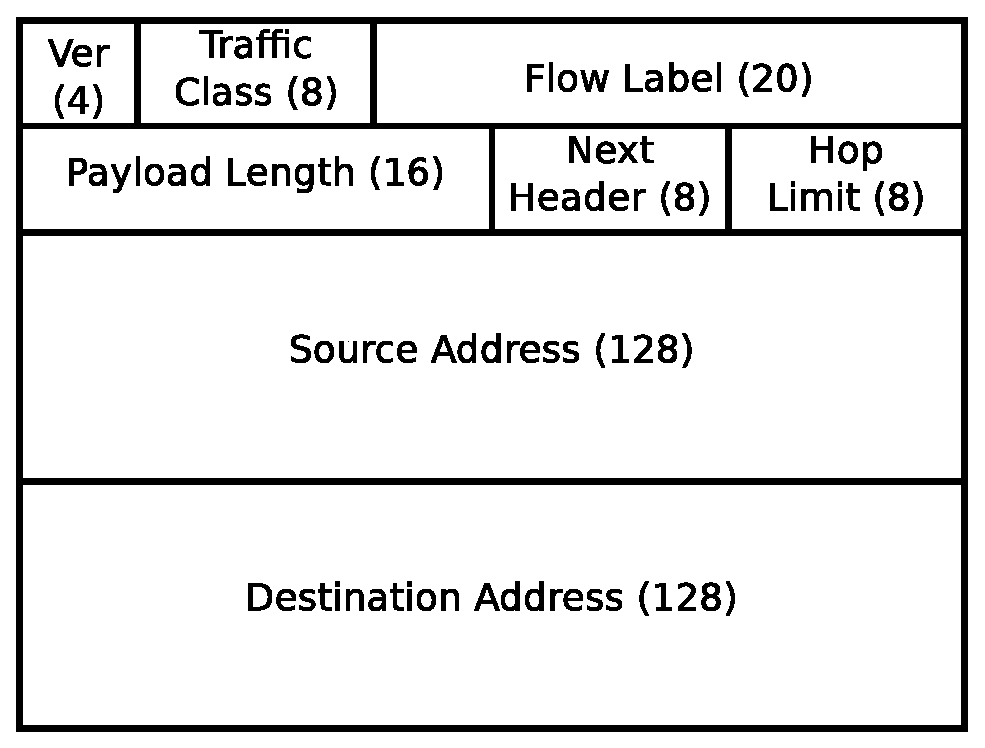
\includegraphics[width=4in]{IPv6_header}
\caption{L'en-tête IPv6}
\label{fig:IPv6}
\end{figure}

\begin{table}[htb]
\caption{Plages de valeurs pour le champ \texttt{DSCP}}
\centering
\begin{tabular}{|c|c|l|}
\hline\rowcolor[gray]{0.8}\color{black}
Plage & Valeurs & Règle d'assignation\\\hline
1 & xxxxx0 & Assignation par une norme de l'IANA\\\hline
2 & xxxx11 & Expérimentation/Usage local\\\hline
3 & xxxx01 & Expérimentation/Usage local (pourrait être jointe à la plage 1)\\\hline
\end{tabular}
\label{tab:RangesDSCP}
\end{table}

% On veut éviter que la figure et le tableau soient placés au-delà de la section courante.
% To prevent the figure and table from being positioned outside of the current section. 
\FloatBarrier


%%
%% OBJECTIFS DE RECHERCHE / RESEARCH OBJECTIVES
%%
\section{Objectifs de recherche}  % 0.5 page
Les objectifs de la recherche sont de concevoir un algorithme $O(n)$.


%%
%% PLAN DU MEMOIRE / THESIS OUTLINE
%%
\section{Plan du mémoire}  % 0.5 page

Voir la Figure~\ref{fig:Layers} pour plus de détails. 

\begin{figure}[htb]
\centering
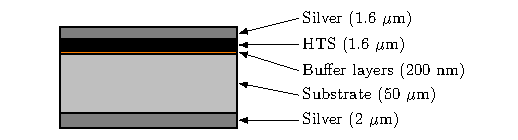
\includegraphics[width=4in]{demo_tikz}
\caption{Couches}
\label{fig:Layers}
\end{figure}


Un tableau : / A table:
\begin{table}[htb]
  \centering
  \caption{Constantes et variables du modèle analytique}
  \begin{tabular}{|c|l|}
    \hline\rowcolor[gray]{0.8}\color{black}
    Symbole         & Description\\\hline
    $\lambda$       & Taux d'arrivée moyen des requêtes de réservation de ressources\\\hline
    $\frac{1}{\mu}$ & Durée moyenne d'une session\\\hline
    $C$             & Capacité d'une cellule (nombre de sessions supportées)\\\hline
    $v_{moy}$       & Vitesse moyenne des MN dans le réseau d'accès\\\hline
    $L$             & Longueur d'un côté d'une cellule carrée\\\hline
    $n$             & Nombre moyen de MN dans une cellule\\\hline
    $\rho$          & Charge d'une cellule\\\hline
    $P_b$           & Probabilité de blocage d'une requête de réservation\\\hline
    $P_f$           & Probabilité d'interruption forcée d'une session\\\hline
    $P_c$           & Probabilité de compléter une session avec succès\\\hline
    $\Delta{}T$     & Délai de transmission\\\hline
  \end{tabular}
  \label{tab:Definitions}
\end{table}

La formule d'\mbox{Erlang-B}:
\begin{equation}
  P_b = \frac{\frac{\rho^C}{C!}}{\sum\limits_{x=0}^{C}\frac{\rho^x}{x!}}
  \label{eq:Pblock}
\end{equation}

Une autre équation : / Another equation:
\begin{equation}
  \begin{split}
    P_c &= (1 - P_b) \times (1 -  P_f)^N\\
        &= (1 - P_b)^{N+1}
  \end{split}
  \label{eq:ProbComplete}
\end{equation}

Enfin, l'expression suivante indique le moment à partir duquel les
réservations de ressources sont en place:
\begin{equation}
  \Delta{}T_{init} =
  \begin{cases}
    2\Delta{}T_{E2E} & \Delta{}T_{wan} > (\Delta{}T_{rad} + \Delta{}T_{net})\\
    \Delta{}T_{E2E} + 3(\Delta{}T_{rad} + \Delta{}T_{net}) & \text{sinon}
  \end{cases}
  \label{eq:InitCost}
\end{equation}

\paragraph{Le taux de paquets perdus} correspond au nombre de paquets
éliminés à cause d'une erreur de \emph{checksum} à un n\oe{}ud
quelconque ou d'une situation de congestion. Le taux de paquets perdus
pour un chemin est déterminé de la façon suivante:
\begin{equation}
  \label{eq:genPLR}
  PLR_P = 1 - \prod_{i=1}^N(1 - PLR_i)
\end{equation}

Toutefois, si les taux d'erreurs sont très faibles, comme c'est
généralement le cas pour des liens optiques, on peut approximer
$PLR_P$ de façon à le transformer en un paramètre additif:
\begin{equation}
  \label{eq:approxPLR}
  \begin{split}
    PLR_{L_1 \oplus L_2} &= 1 - (1 - PLR_1)(1 - PLR_2)\\
    &= 1 - (1 - PLR_2 - PLR_1 + \underbrace{PLR_1
      \times PLR_2}_\text{négligeable})\qquad PLR_1 \ll 1,
    PLR_2 \ll 1\\
    &\approx PLR_1 + PLR_2
  \end{split}
\end{equation}

\clearpage

Une courbe : / A curve:
\begin{figure}[htb]
\centering
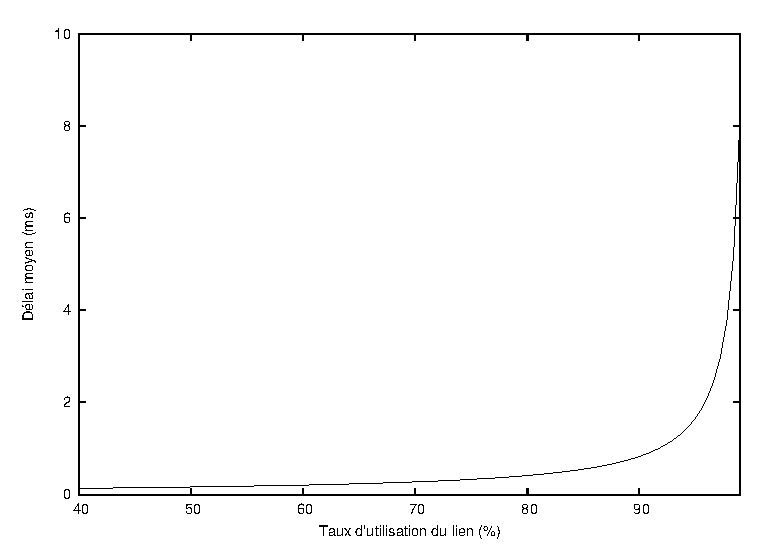
\includegraphics[width=5in]{LinkUsage}
\caption{Délai moyen en fonction du taux d'utilisation d'un lien}
\label{fig:LinkUse}
\end{figure}

\selectlanguage{english}
This paragraph is formatted by \LaTeX{} according to the standard rules of the
English language (\mbox{e.g.} hyphenation).
\selectlanguage{french}

L'arithmétique en virgule flottante peut entraîner des erreurs
d'approximation et il est important d'en être conscient
\cite{Rossi2011}.

De même, les calculs effectués sur une carte graphique (GPU) peuvent
introduire des erreurs d'approximation \cite{DeSantis2002, Cohen2006,
  Thorsson2014, Schirmer2012, Sakai2015, Electrical2006,
  Min2016, Massicotte2013, Kaliouby1987, Daintith2010, Haist2014, Kizza2013,
  Manasreh2011, Brydson1999, Boyce2002}.
